\documentclass[a4paper,14pt]{extarticle}

\usepackage[T2A]{fontenc}			
\usepackage[utf8]{inputenc}			
\usepackage[english,russian]{babel}

\usepackage[
bookmarks=true, colorlinks=true, unicode=true,
urlcolor=black,linkcolor=black, anchorcolor=black,
citecolor=black, menucolor=black, filecolor=black,
]{hyperref}

\usepackage{color}
\usepackage{caption}
\DeclareCaptionFont{white}{\color{black}}
\DeclareCaptionFormat{listing}{\colorbox{white}{\parbox{\textwidth}{#1#2#3}}}
\captionsetup[lstlisting]{format=listing,labelfont=white,textfont=white}

\usepackage{amsmath,amsfonts,amssymb,amsthm,mathtools} 
\usepackage{wasysym}

\usepackage{graphicx}
%\usepackage[cache=false]{minted}
\usepackage{cmap}
\usepackage{indentfirst}

\usepackage{listings} 
\usepackage{fancyvrb}

\usepackage{geometry}
\geometry{left=2cm}
\geometry{right=1.5cm}
\geometry{top=1cm}
\geometry{bottom=2cm}

\setlength{\parindent}{5ex}
\setlength{\parskip}{0.5em}

\usepackage{color}
\usepackage[cache=false, newfloat]{minted}
\newenvironment{code}{\captionsetup{type=listing}}{}
\SetupFloatingEnvironment{listing}{name=Листинг}
 
 
 \begin{document}
 	
 	\def\figurename{Рисунок}
 	
 	\begin{minipage}{0.2\textwidth}
 		
\includegraphics[scale=0.05]{img/bmstu.png}
 	\end{minipage}
 	\begin{minipage}{0.7\textwidth}
 		\small
 		\begin{center}
 			\textbf{Министерство науки и высшего образования Российской Федерации}
 			
 			\textbf{Федеральное государственное бюджетное образовательное учреждение высшего образования «Московский государственный технический университет имени Н.Э. Баумана}
 			
 			\textbf{(национальный исследовательский университет)»}
 			
 			\textbf{(МГТУ им. Н.Э. Баумана)}
 		\end{center}
 	\end{minipage}
 	
 	\vspace*{5mm}
 	
 	\vspace*{30mm}
 	
 	\LARGE
 	\begin{center}
 		\textbf{Рубежный контроль №3}
 		
 		%	\textbf{к курсовому проекту на тему:}
 		\textbf{Реферат на тему:}
 		
 		\textbf{<<Методы и технологии управления инновационными проектами.>>}
 	\end{center}
 	
 	%\huge
 	%\begin{center}
 	%	\textbf{Лабораторная работа №9}
 	%\end{center}
 	%
 	%\begin{center}
 	%	\textbf{Тема:} <<Обработчики прерываний>>
 	%\end{center}
 	
 	\vspace*{15mm}
 	
 	\large
 	\begin{flushleft}
 		\textbf{Дисциплина:} Экономика \\
 		\textbf{Студент:} Левушкин И. К. \\
 		\textbf{Группа:} ИУ7-72Б \\
 		%        \textbf{Оценка (баллы):} \\
 		\textbf{Преподаватель:} Герцик Ю.Г.\\
 	\end{flushleft}
 	
 	\vspace*{50mm}
 	
 	\large
 	\begin{center}
 		Москва, 2020 г.
 	\end{center}
 	
 	\thispagestyle{empty}
 	
 	\newpage
 	
 	\tableofcontents
 	\newpage
 	\section*{Введение}
 	\addcontentsline{toc}{section}{Введение}
 	
 	У человечества за всю историю накопился внушительный список успешно реализованных сложных проектов. От строительства Пирамид в Гизе до отправки человека на Луну, самые смелые человеческие начинания требовали слаженной работы тысяч людей. А это подразумевает сложную систему управления проектами.
 	
 	Управление проектами – это управление и организация всего, что нужно для достижения цели – вовремя и в рамках бюджета. Будь то разработка нового программного обеспечения, проведение маркетинговой компании или высадка человека на Марс – проектное управление позволяет добиться успеха.
 	
 	Все проекты разные. Не существует идеальной системы управления проектами, подходящей для каждого из видов проектов. Также не существует системы, которая бы подходила каждому руководителю и была удобна для всех членов команды. Однако за время существования проектного управления было создано немало эффективных подходов, методик и стандартов, которые можно взять на вооружение.
 	
 	\newpage
 	
 	\section{Водопадная модель}
 	
 	Наиболее очевидным способом управления проектами выступает разделение процесса исполнения того или иного проекта на ряд последовательных этапов. Именно линейная структура является базой осуществления традиционного проектного управления. 
 	
 	Классический водопадный метод управления проектами предусматривает выделение следующих этапов: 
 	\begin{enumerate}
 		\item этап инициации. На этом этапе определяются требованиями к проекту. Для этапа характерно проведение совещаний и «мозговых штурмов», результатом которых становится предполагаемый продукт проекта; 
 		\item этап планирования. Данный этап характеризуется определением того, как будет осуществляться достижение цели, определенной ранее. Команда проекта осуществляет уточнение и детализацию целей и результатов проекта, определяет состав работ. Данная информация выступает основой формирования календарного плана и бюджета, оценки рисков и выявления заинтересованных лиц; 
 		\item этап разработки. Реализация данного этапа осуществляется не у всех проектов, поскольку зачастую он является частью этапа планирования. Наиболее характерно наличие этого этапа для технологических проектов. Данный этап предназначен для определения конфигурации проекта и его продуктов, а также технических способов достижения необходимого результата; 
 		\item этап реализации и тестирования. Этот этап включает в себя основную работу по проекту, то есть непосредственное создание продукта. В ИТ-проектах это может быть написание кода, в строительных – возведение сооружений и так далее. Суть этого этапа состоит в реализации разработанных планов проекта, осуществлении контроля определенных показателей. Также на этом этапе проект подвергается тестированию на соответствие требованиям. Результатом тестирования является выявление недостатков и их исправление; 
 		\item этап мониторинга и завершения проекта. Содержание данного этапа управления проектами может различаться в зависимости от сложности проекта. В определенных случаях этот этап может включать в себя просто передачу заказчику продукта проекта. В другом случае речь идет о длительном процессе взаимодействия с заказчиком, направленном на улучшение проекта и повышение степени удовлетворенности его результатом.
 	\end{enumerate}
 
 	Классический метод управления проектами составляет основу для всех других методов управления проектами. Данный метод применяется по отношению к проектам, которые имеют строгие ограничения относительно последовательности их исполнения.
 	
 	\textit{Основным преимуществом} данного метода является то, что заказчик и исполнитель еще на первом этапе определяют, какой результат они хотят получить. Это является основой стабильности при осуществлении управления проектом, фундаментом упорядочения процесса его реализации.
 	
 	\textit{Основным недостатком} данного метода является отсутствие толерантности к изменениям. В настоящее время применение классического метода управления проектами в наибольшей мере относится к строительным и инженерным проектам.
 	
 	\section{V-модель}
 	
 	V-модель – это улучшенная версия классической каскадной модели. Здесь на каждом этапе происходит контроль текущего процесса, для того чтобы убедится в возможности перехода на следующий уровень. В этой модели тестирование начинается еще со стадии написания требований, причем для каждого последующего этапа предусмотрен свой уровень тестового покрытия.
 	
 	Для каждого уровня тестирования разрабатывается отдельный тест-план, то есть во время тестирования текущего уровня, происходит разработка стратегии тестирования следующего. при создавании тест-планов,определяются ожидаемые результаты тестирования и указываются критерии входа и выхода для каждого этапа.
 	
 	В V-модели каждому этапу проектирования и разработки системы соответствует отдельный уровень тестирования. Здесь процесс разработки представлен нисходящей последовательностью в левой части условной буквы V, а стадии тестирования – на ее правом ребре. Соответствие этапов разработки и тестирования показано горизонтальными линиями.
 	
 	\textit{Основные преимущества V-модели разработки}
 	\begin{itemize}
 		\item строгая этапизация;
 		\item планирование тестирования и верификация системы производятся на ранних этапах;
 		\item улучшенный, по сравнению с каскадной моделью, тайм-менеджмент;
 		\item промежуточное тестирование.
 	\end{itemize}
 
 	\textit{Основные недостатки V-модели разработки}
 	\begin{itemize}
 		\item недостаточная гибкость модели;
 		
 		\item собственно создание программы происходит на этапе написания кода, то есть уже в середине процесса разработки;
 		
 		\item недостаточный анализ рисков;
 		
 		\item нет работы с параллельными событиями и возможности динамического внесения изменений.
 	\end{itemize}
 
 	V-модель используется:
 	\begin{itemize}
 		\item В проектах, в которых существуют временные и финансовые ограничения;
 		
 		\item Для задач, которые предполагают более широкое, по сравнению с каскадной моделью, тестовое покрытие.
 	\end{itemize}
 	
 	\section{Итеративная модель}
 	
 	Итеративная разработка ПО — это процесс создания программного обеспечения, который осуществляется небольшими этапами, в ходе которых ведется анализ полученных промежуточных результатов, выдвигаются новые требования и корректируются предыдущие этапы работы.
 	
 	Жизненный цикл проекта при итерационной разработке разбит на последовательность итераций, каждая из которых, по сути, является проектом в миниатюре, то есть включает в себя все процессы разработки ПО (сбор и анализ требований, составление спецификаций, непосредственную реализацию, тестирование и запуск), но в рамках одной итерации разрабатывается не весь проект, а только его версия или отдельная часть.
 	
 	Как правило, цель каждой итерации — это получение версии ПО, включающей в себя как новые или преработанные возможности, реализованные в ходе текущей итерации, так и функциональность всех предыдущих итераций. Результат же финальной итерации содержит всю требуемую функциональность продукта.
 	
 	Бюджет и сроки, необходимые для реализации финальной версии обычно изначально не устанавливаются, так как не определяется общий объём работ и требования формируются по ходу реализации.
 	
 	\textit{Основные преимущества итеративной модели разработки}
 	
 	\begin{itemize}
 		\item Снижение рисков — раннее обнаружение конфликтов между требованиями, моделями и реализацией проекта; большая фокусировка на основных задачах; динамическое формирование требований и управление ими.
 		
 		\item Организация эффективной обратной связи проектной команды с потребителем, создание продукта, реально отвечающего его потребностям.
 		
 		\item Быстрый выпуск минимально ценного продукта (MVP) и возможность вывести продукт на рынок и начать эксплуатацию гораздо раньше.
 	\end{itemize}
 	
 	\textit{Основные недостатки итеративной модели разработки}
 	
 	\begin{itemize}
 		\item Проблемы с архитектурой и накладные расходы — при работе с хаотичными требованиями и без проработанного глобального плана архитектура приложения может пострадать, а на её приведение к адекватному виду могут потребоваться дополнительные ресурсы. По сути, за возможность менять требования в ходе создания продукта, приходится так или иначе расплачиваться.
 		
 		\item Нет фиксированного бюджета и сроков, а также нужна сильная вовлеченность Заказчика в процесс — для некоторых Заказчиков это неприемлемые условия сотрудничества с разработчиком, им лучше подойдёт водопадная модель.
 	\end{itemize}
 
 	Итеративная модель используется:
 	\begin{itemize}
 		\item В больших проектах;
 		\item В проектах с неопределенными требованиями;
 		\item В проектах, которые носят инновационный характер и основаны на бизнес-гипотезах, требующих проверки.
 	\end{itemize}
 	
 	\section{Спиральная модель}
 	
 	{\bf Спиральную модель}  можно описать как повторяющуюся последовательность циклов разработки с непрерывным контролем рисков.
 	
 	Ниже приведена схема механизма разработки ПО, использующая спиральную модель.
 	
 	\begin{figure}[h!]
 		\begin{center}
 			{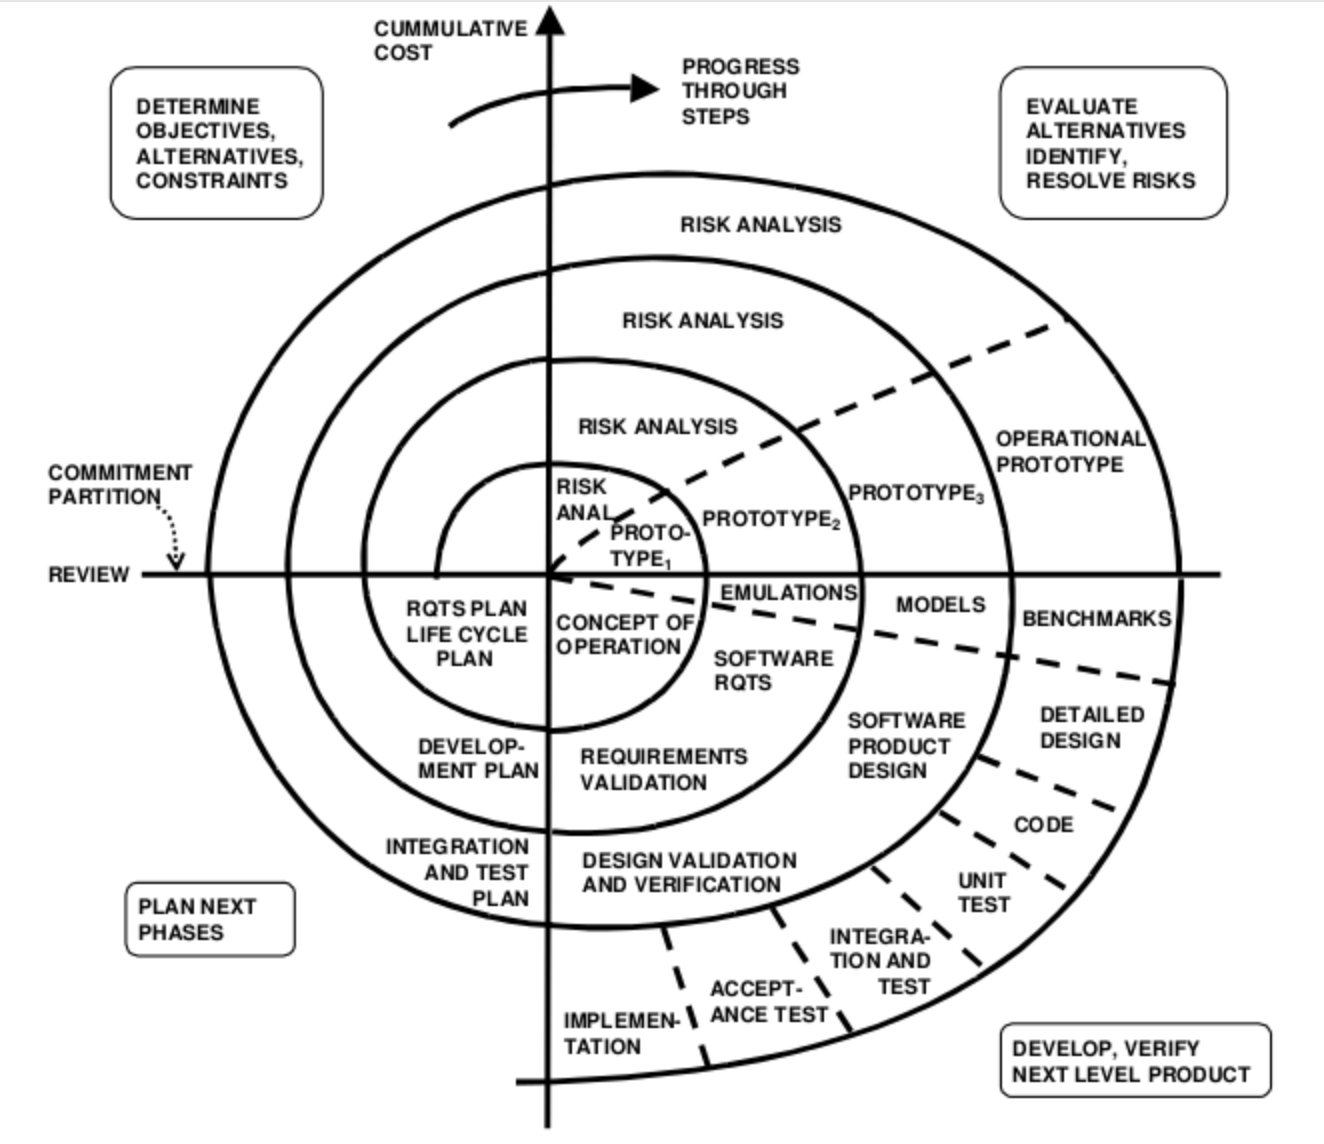
\includegraphics[scale = 0.4]{spiral.png}}
 			\label{ris:spiral}
 		\end{center}
 		\caption{Спиральная модель.}
 	\end{figure}
 
 	Исходя из схемы, видно, что спиральная модель состоит из четырех главных повторяющихся стадий. В ходе процесса разработки проект несколько раз проходит через все эти фазы. Каждая такая итерация называется \textit{спиралью}.
 	
 	Четыре главные фазы это:
 	
 	\begin{enumerate}
 		\item {\bf Определение целей, альтернатив, ограничений, или фаза планирования.} С этой стадии начинается работа над проектом. Команда разработчиков формулирует цели проекта, основные требования (такие как, например, Business Requirement Specifications, или BRS, System Requirement Specifications, или SRS), возможный дизайн и т.д. На последующих спиралях требования формируются согласно отзывам, полученным от заказчика. Именно поэтому постоянная коммуникация между заказчиком и командой крайне важна.
 		\item {\bf Анализ, определение и разрешение рисков} является одной из самых значимых стадий разработки. В данном контексте,  риски — это возможные события и состояния проекта, препятствующие достижению командой разработчиков поставленных целей. Существует довольно обширный диапазон возможных рисков, от тривиальных и легко преодолимых, до крайне серьезных. Главной задачей для команды разработчиков является выявление всех возможных рисков и присвоение им определенного уровня приоритета на основе их значимости. Следующим шагом является разработка возможных стратегий преодоления этих рисков. В итоге этих действий возможны изменения в последующих стадиях разработки. В качестве результата работы на этом этапе создается прототип.
 		\item {\bf Фаза разработки.} На этом этапе происходит разработка и последующее тестирование продукта. Во время первой итерации, когда общие требования еще не так четко сформулированы, разрабатывается так называемый концепция будущего продукта (Proof Of Concept), которая необходима для получения отзыва заказчика. На последующих витках спирали рабочие версии продукта, или билды (builds), отправляются заказчику. Это позволяет получить более детальный отзыв и четче сформулировать требования.
 		\item {\bf Планирование следующей фазы.} На этом этапе вся полученная информация используется для планирования дальнейших этапов разработки.
 	\end{enumerate}
 	
 	\textit{Основные преимущества спиральной модели разработки}
 	
 	\begin{itemize}
 		\item Мониторинг рисков является одной из главных особенностей, делающих данную модель особенно привлекательной в том случае, если вам предстоит управление большим, сложным и дорогостоящим проектом. Более того, проект будет более прозрачным, поскольку спиральная модель изначально была спроектирована таким образом, чтобы каждая итерация тщательно анализировалась;
 		\item Заказчик может увидеть работающую версию продукта уже на ранних стадиях жизненного цикла ПО;
 		\item Изменения могут быть внесены на поздних стадиях разработки;
 		\item Проект может быть разделен на несколько частей и те из них, которые, согласно анализу, окажутся более рискованными, могут быть реализованы на ранних стадиях. Такой подход может снизить трудности, связанные с управлением проектом;
 		\item Строгий контроль над документацией, как результат постоянного анализа рисков.
 	\end{itemize}
 	
 	\textit{Основные недостатки спиральной модели разработки}
 	
 	\begin{itemize}
 		\item Мониторинг рисков требует дополнительных ресурсов, а значит, эта модель может оказаться весьма затратной. Каждая итерация требует отдельной экспертизы, что делает управление проектом сложнее. Именно поэтому спиральная модель плохо подходит для небольших проектов;
 		\item Большое количество промежуточных стадий разработки. Как следствие — большой объем документации;
 		\item На самых ранних стадиях дата завершения работы над проектом может быть неизвестна, что также усложняет контроль над процессом разработки
 	\end{itemize}
 
 	Спиральная модель используется в проектах, где:
 	\begin{itemize}
 		\item предстоит работа со средним или высоким уровнем возможных рисков;
 		\item заказчик не может предоставить достаточно четкий список требований к конечному продукту или эти требования достаточно сложные;
 		\item ожидаются значительные изменения в процессе разработки.
 	\end{itemize}
 	
 	\section{Agile}
 	
 	{\bf Agile} — итеративная модель разработки, в которой программное обеспечение создают инкрементально с самого начала проекта, в отличии от каскадных моделей, где код доставляется в конце рабочего цикла.
 	
 	Основа гибкой методологии — разбиение проектов на маленькие рабочие кусочки, называемые пользовательскими историями. Согласно приоритетности задачи решают в рамках коротких двухнедельных циклов (итераций).
 	
 	12 принципов, которые составляют Agile Methodology, можно поделить на 4 главные идеи:
 	
 	\begin{itemize}
 		\item Приоритет людей и общения над инструментами и процессами;
 		\item Приоритет работающего продукта над полной документацией;
 		\item Приоритет сотрудничества с заказчиков над утверждением контракта;
 		\item Приоритет готовности меняться над следованием первоначально созданному плану.
 	\end{itemize}
 
 	Эти идеи раскрываются в 12 принципах Agile Manifesto:
 	
 	\begin{enumerate}
 		\item работающий конкурентоспособный продукт, удовлетворяющий заказчика — лучший показатель прогресса и измеритель эффективности;
 		\item оперативная и бесперебойная поставка продукта, удовлетворяющего заказчика;
 		\item адаптивность продукта к новым требованиям, которые могут повысить его ценность и конкурентоспособность (возможность внесения изменений на любом этапе разработки);
 		\item простота и прозрачность технических решений, документации, процессов и инструментов, чтобы не создавать лишней работы;
 		частая поставка функционирующего продукта (раз в месяц/неделю или ещё чаще);
 		\item постоянный темп работы всех участников проекта на протяжении всего его срока;
 		\item минимизация организационных и информационных барьеров, лучший путь передачи информации — это личный разговор лицом к лицу;
 		\item тесное и ежедневное общение исполнителей с заказчиком в течении всего проекта;
 		\item мотивация участников проекта и обеспечение их всеми необходимыми условиями работы, поддержкой и доверием;
 		\item самоорганизация и самоконтроль команды проекта;
 		\item непрерывное улучшение профессиональных компетенций команды проекта;
 		\item систематический анализ и постоянный поиск возможностей оптимизации командной и индивидуальной работы.
 	\end{enumerate}
 
 	\textit{Основные преимущества agile-модели разработки}
 	
 	\begin{itemize}
 		\item быстрота, адаптивность и фокус на главном;
 		\item Отсутствие бюрократии и периодичность поставок работающего продукта с постепенным наращиванием его функциональных возможностей.
 	\end{itemize}
 	
 
 	\textit{Основные недостатки agile-модели разработки}
 	
 	\begin{itemize}
 		\item снижение важности регламентирующей и технической документации может привести к ее нерелевантности или даже к фактическому отсутствию;
 		\item краткосрочное планирование не всегда учитывает необходимость масштабирования продукта, что влечет ошибки в архитектуре;
 		\item появление новых требований после нескольких итераций приводит к кардинальным изменениям архитектуры и переделкам уже созданных решений;
 		\item накопление дефектов и снижение качества продуктов вследствие решения проблем самым простым и быстрым, но не всегда самым правильным способом.
 	\end{itemize}
 	
 	Agile-модель используется не только в управлении ИТ-проектами, а используется как эффективная практика организации труда небольших групп и творческих команд вместе с либеральными и демократическими методами менеджмента.
 	
 	
 	\newpage
 	\section{Заключение}
 	\addcontentsline{toc}{section}{Заключение}
 	
 	В данной работе был проведен анализ наиболее популярных методов и технологий, используемых для управления инновационными проектами. 
 	
 	Были даны основные положения каждого из методов, разобраны их преимущества и недостатки, а также место их применения.
 	
 	В итоге, поставленная цель, заключающаяся в исследовании
 	методов и технологий управления инновационными проектами, достигнута.
 	
 	\newpage
 	
 	
 	\addcontentsline{toc}{section}{Список используемой литературы}
 	\begin{thebibliography}{3}
 		\bibitem{first}
 		Основные методологии разработки [Электронный ресурс]. – Режим доступа: 
 		https://habr.com/ru/company/edison/blog/269789/, 
 		свободный – (11.12.2020)
 		\bibitem{second} Проектный менеджмент
 		в IT - как это? [Электронный ресурс]. – Режим доступа: 
 		https://worksection.com/blog/it-project-management.html, 
 		свободный – (11.12.2020)
 		\bibitem{third} Топ-7 методов управления проектами: Agile, Scrum, Kanban, PRINCE2 и другие [Электронный ресурс]. – Режим доступа: 
 		https://www.pmservices.ru/project-management-news/top-7-metodov-upravleniya-proektami-agile-scrum-kanban-prince2-i-drugie/, 
 		свободный – (11.12.2020)
 	\end{thebibliography}
 	
 \end{document}